\RequirePackage[dvipsnames,prologue,table]{xcolor}
\documentclass[pstricks]{standalone}
\usepackage{pst-text}
\usepackage{pst-grad}
\usepackage{graphicx}
\usepackage{lipsum}
\usepackage{svg}

\setlength{\parindent}{0ex}

\begin{document}
\pagestyle{empty}

% create the box with the front cover picture
%\newsavebox\IBox
%\sbox\IBox{\includegraphics[height=11.250in]{by-sa.eps}}

% set up the picture environment
\psset{unit=1in}
\begin{pspicture}(17.407in,11.250in)

% set up the fonts we use
\DeclareFixedFont{\PT}{T1}{ppl}{b}{n}{0.7in}
\DeclareFixedFont{\PTsmall}{T1}{ppl}{b}{n}{0.4in}
\DeclareFixedFont{\PTsmallest}{T1}{ppl}{b}{n}{0.3in}
\DeclareFixedFont{\PTtext}{T1}{ppl}{b}{it}{11pt}


\psframe[fillstyle=solid,fillcolor=Goldenrod,linecolor=Goldenrod,dimen=outer](0,0)(8.7035,11.250)
\psframe[fillstyle=solid,fillcolor=Turquoise,linecolor=Turquoise,dimen=outer](8.7035,0)(17.407,11.250)

% put the text on the front cover
\newsavebox\Titlebbox
\sbox\Titlebbox{\begin{minipage}{6in} \centering
\lineskip=10pt
\PT \textcolor{white}{12 Partitions pour\\\mbox{Xylophone}\\ \&\\ \mbox{Métallophone}\\ à 8 barres}
\end{minipage}}

% And position the box
\rput[t](13.05525,10){\usebox\Titlebbox}
\rput[t](13.05525,5){\PTsmall \color{white}{Guilhem Vellut}}

\newsavebox\IBox
\sbox\IBox{\includesvg{xylophone.svg}}

\rput[lb](7.24,0){\usebox\IBox}

\newsavebox\Contentbbox
\sbox\Contentbbox{\begin{minipage}{8in} \centering
\lineskip=15pt
\baselineskip=15pt
\lineskiplimit=15pt
\PTsmallest \color{white}
Au clair de la lune\newline
\par
L'alphabet\newline
\par
\baselineskip=10pt
À la claire fontaine\newline
\par
\baselineskip=15pt
Pirouette Cacahuète\\
Dansons la capucine\newline
Il court, il court, le furet\\
Promenons-nous dans les bois\\
Vive le vent\\
Frère Jacques\newline
Bonjour, belle Rosinne\newline
À la pêche aux moules\\
Le roi Dagobert
\par
\end{minipage}}
\rput[t](4.35175,10){\usebox\Contentbbox}


\psframe[fillstyle=solid,fillcolor=Lavender,linecolor=Lavender,dimen=outer](0,0)(0.58023333,3.0)
\psframe[fillstyle=solid,fillcolor=ProcessBlue,linecolor=ProcessBlue,dimen=outer](0.58023333,0)(1.16046667,3.0)
\psframe[fillstyle=solid,fillcolor=Rhodamine,linecolor=Rhodamine,dimen=outer](1.16046667,0)(1.7407,3.0)
\psframe[fillstyle=solid,fillcolor=RubineRed,linecolor=RubineRed,dimen=outer](1.7407,0)(2.32093333,3.0)
\psframe[fillstyle=solid,fillcolor=BrickRed,linecolor=BrickRed,dimen=outer](2.32093333,0)(2.90116667,3.0)
\psframe[fillstyle=solid,fillcolor=CadetBlue,linecolor=CadetBlue,dimen=outer](2.90116667,0)(3.4814,3.0)
\psframe[fillstyle=solid,fillcolor=CornflowerBlue,linecolor=CornflowerBlue,dimen=outer](3.4814,0)(4.06163333,3.0)
\psframe[fillstyle=solid,fillcolor=RedViolet,linecolor=RedViolet,dimen=outer](4.06163333,0)(4.64186667,3.0)
\psframe[fillstyle=solid,fillcolor=Brown,linecolor=Brown,dimen=outer](4.64186667,0)(5.2221,3.0)
\psframe[fillstyle=solid,fillcolor=WildStrawberry,linecolor=WildStrawberry,dimen=outer](5.2221,0)(5.80233333,3.0)
\psframe[fillstyle=solid,fillcolor=Mahogany,linecolor=Mahogany,dimen=outer](5.80233333,0)(6.38256667,3.0)
\psframe[fillstyle=solid,fillcolor=BlueGreen,linecolor=BlueGreen,dimen=outer](6.38256667,0)(6.9628,3.0)
\psframe[fillstyle=solid,fillcolor=Cerulean,linecolor=Cerulean,dimen=outer](6.9628,0)(7.54303333,3.0)
\psframe[fillstyle=solid,fillcolor=SpringGreen,linecolor=SpringGreen,dimen=outer](7.54303333,0)(8.12326667,3.0)
\psframe[fillstyle=solid,fillcolor=Sepia,linecolor=Sepia,dimen=outer](8.12326667,0)(8.7035,3.0)
\psframe[fillstyle=solid,fillcolor=BurntOrange,linecolor=BurntOrange,dimen=outer](8.7035,0)(9.28373333,3.0)
\psframe[fillstyle=solid,fillcolor=RubineRed,linecolor=RubineRed,dimen=outer](9.28373333,0)(9.86396667,3.0)
\psframe[fillstyle=solid,fillcolor=Cerulean,linecolor=Cerulean,dimen=outer](9.86396667,0)(10.4442,3.0)
\psframe[fillstyle=solid,fillcolor=SkyBlue,linecolor=SkyBlue,dimen=outer](10.4442,0)(11.02443333,3.0)
\psframe[fillstyle=solid,fillcolor=Brown,linecolor=Brown,dimen=outer](11.02443333,0)(11.60466667,3.0)
\psframe[fillstyle=solid,fillcolor=DarkOrchid,linecolor=DarkOrchid,dimen=outer](11.60466667,0)(12.1849,3.0)
\psframe[fillstyle=solid,fillcolor=Maroon,linecolor=Maroon,dimen=outer](12.1849,0)(12.76513333,3.0)
\psframe[fillstyle=solid,fillcolor=Melon,linecolor=Melon,dimen=outer](12.76513333,0)(13.34536667,3.0)
\psframe[fillstyle=solid,fillcolor=MidnightBlue,linecolor=MidnightBlue,dimen=outer](13.34536667,0)(13.9256,3.0)
\psframe[fillstyle=solid,fillcolor=BrickRed,linecolor=BrickRed,dimen=outer](13.9256,0)(14.50583333,3.0)
\psframe[fillstyle=solid,fillcolor=LimeGreen,linecolor=LimeGreen,dimen=outer](14.50583333,0)(15.08606667,3.0)
\psframe[fillstyle=solid,fillcolor=BlueViolet,linecolor=BlueViolet,dimen=outer](15.08606667,0)(15.6663,3.0)
\psframe[fillstyle=solid,fillcolor=ForestGreen,linecolor=ForestGreen,dimen=outer](15.6663,0)(16.24653333,3.0)
\psframe[fillstyle=solid,fillcolor=Peach,linecolor=Peach,dimen=outer](16.24653333,0)(16.82676667,3.0)
\psframe[fillstyle=solid,fillcolor=Sepia,linecolor=Sepia,dimen=outer](16.82676667,0)(17.407,3.0)

\end{pspicture}
\end{document}
